\section{Création de la base de données ontologique}
\subsection{L'ontologie du projet}

\subsubsection{Les ontologies : la théorie}
\paragraph{} \hspace{10mm}
Une ontologie informatique est un modèle conceptuel qui décrit les concepts et les relations qui existent dans un domaine d'application spécifique. Elle sert à fournir une structure de données commune pour les systèmes informatiques qui traitent ces données. Les ontologies informatiques sont généralement définies en utilisant un formalisme de description de la connaissance, comme OWL (Web Ontology Language) ou RDF (Resource Description Framework). Elles peuvent être utilisées pour des tâches comme la classification automatique, la recherche d'information, la reconnaissance de la parole, la compréhension de la langue naturelle, et la communication entre systèmes informatiques.
Elles sont utilisées pour fournir un cadre commun pour les systèmes informatiques pour comprendre et partager l'information. Cela permet de faciliter la communication entre les systèmes et d'améliorer l'interopérabilité entre différents systèmes. Elles sont également utilisées pour améliorer la performance des systèmes d'IA en fournissant une description précise et complète des concepts dans un domaine d'application.

\paragraph{} \hspace{10mm}
Cette approche étant plutôt abstraite, on peut la concrétiser en ajoutant que le World Wide Web Consortium a défini un langage appelé OWL (Web Ontology Language) basé sur le standard RDF (Resource Description Framework). RDF est un framework permettant de modéliser des graphes destiné à décrire des ressources web (et leurs métadonnées). Un document suivant la structure RDF est composé de \textbf{triplets} ordonnés de la manière suivante : \textbf{(sujet, prédicat, objet)}.

\begin{itemize}
    \item[\ding{103}] Le \textbf{sujet} est la ressource que l'on souhaite décrire.
    \item[\ding{103}] Le \textbf{prédicat} est la propriété que l'on souhaite appliquer sur le sujet.
    \item[\ding{103}] L'\textbf{objet} est la ressource ou la valeur litérale (nombre, chaine de caractères, URI) que l'on associe au sujet. Autrement dit, c'est la valeur de la propriété.
\end{itemize}

Voici un court exemple résumant l'aspect théorique. Imaginons que l'on veuille représenter des données et métadonnées de la page wikipédia de \href{https://fr.wikipedia.org/wiki/Johann_Joachim_Winckelmann}{Johann Joachim Winckelmann} à l'aide de l'ontologie \textbf{dcterms}, cela pourrait donner les triplets suivants :
            \begin{minted}{turtle}
            @prefix dcterms: <http://purl.org/dc/terms/>
            
            <https://fr.wikipedia.org/wiki/Johann_Joachim_Winckelmann>
                dcterms:title "Johann Joachim Winckelmann ;
                dcterms:publisher <https://fr.wikipedia.org/> ;
                dcterms:issued 2004-10-19 .
            \end{minted}

\subsubsection{Le modèle ontologique}
\paragraph{} \hspace{10mm}
L'ontologie du projet est basée sur plusieurs ontologies différentes afin de couvrir tous les aspects de la description de patrimoine industriel. La principale ontologie utilisée est celle du \textbf{CIDOC-CRM}, car elle est spécifiquement conçue pour décrire des objets et des événements liés au patrimoine industriel. Nous avons également utilisé  \textbf{Bibo} pour représenter les documents, images et autres sources utilisées dans le projet. Pour décrire les liens entre les personnes morales et physiques ainsi que les groupes de personnes, nous avons utilisé les "sous-ontologies" \textbf{rdac} et \textbf{rdaa}, les deux étant intimement liées : la première regroupe les classes de l'ontologie \textbf{RDA} et la seconde les propriétés qui s'appliquent sur ces classes. Nous avons également utilisé \textbf{dcterms} pour décrire les métadonnées des entités bibo. Enfin, nous avons utilisé \textbf{schema} et \textbf{relationship} pour ajouter quelques propriétés supplémentaires qui ne sont pas couvertes par les ontologies cidoc-crm et rdaa. Cette combinaison d'ontologies permet de couvrir l'ensemble des aspects de la description de patrimoine industriel de manière complète et précise. De plus, il est tout à fait possible de greffer de nouvelles ontologies au besoin dans le cas où les ontologies ici décrites ne suffiraient pas à représenter certaines données ou situations.
\paragraph{} \hspace{10mm}
Dans le cadre du projet, nous n'avons pas ajouté de contenu fait par nous-même (classes ou propriétés) ni modifié en profondeur les ontologies existantes. Cela a été fait pour faciliter l'inter-opérabilité avec d'autres systèmes et garder une ontologie la plus proche possible des normes W3C (World Wide Web Consortium). En utilisant des ontologies existantes et en les combinant de manière appropriée, nous avons pu créer une ontologie personnalisée qui répond aux besoins spécifiques de notre projet tout en restant conforme aux normes de l'industrie. Cela a également permis de réduire les risques d'incompatibilité et faciliter la communication et l'intégration future dans d'autres systèmes.

Pour pouvoir faire ceci de la meilleure manière possible, nous avons, avec Cyril Lachèze et Matthieu Quantin, étudié des cas concrets en utilisant des documents fournis par Cyril. Cela nous a aidé à comprendre comment articuler toutes les ontologies et ainsi élaborer une stratégie pour les combiner efficacement en une seule ontologie globale. Cette approche nous a également permis de mieux comprendre les avantages et les limites de chaque ontologie et de prendre des décisions éclairées sur la façon de les utiliser.

\paragraph{} \hspace{10mm}
Afin de pouvoir dresser le schéma de l'\underline{\hyperref[annexe1]{annexe 1}}, nous avons utilisé des images de l'usine SACM de Belfort que Cyril avait à sa disposition. L'intérêt d'utiliser des cas concrets est que l'on peut couvrir et imaginer comment représenter certains cas d'utilisation que l'on n'aurait pas pu imaginer seul.

\begin{figure} [H]
    \centering
    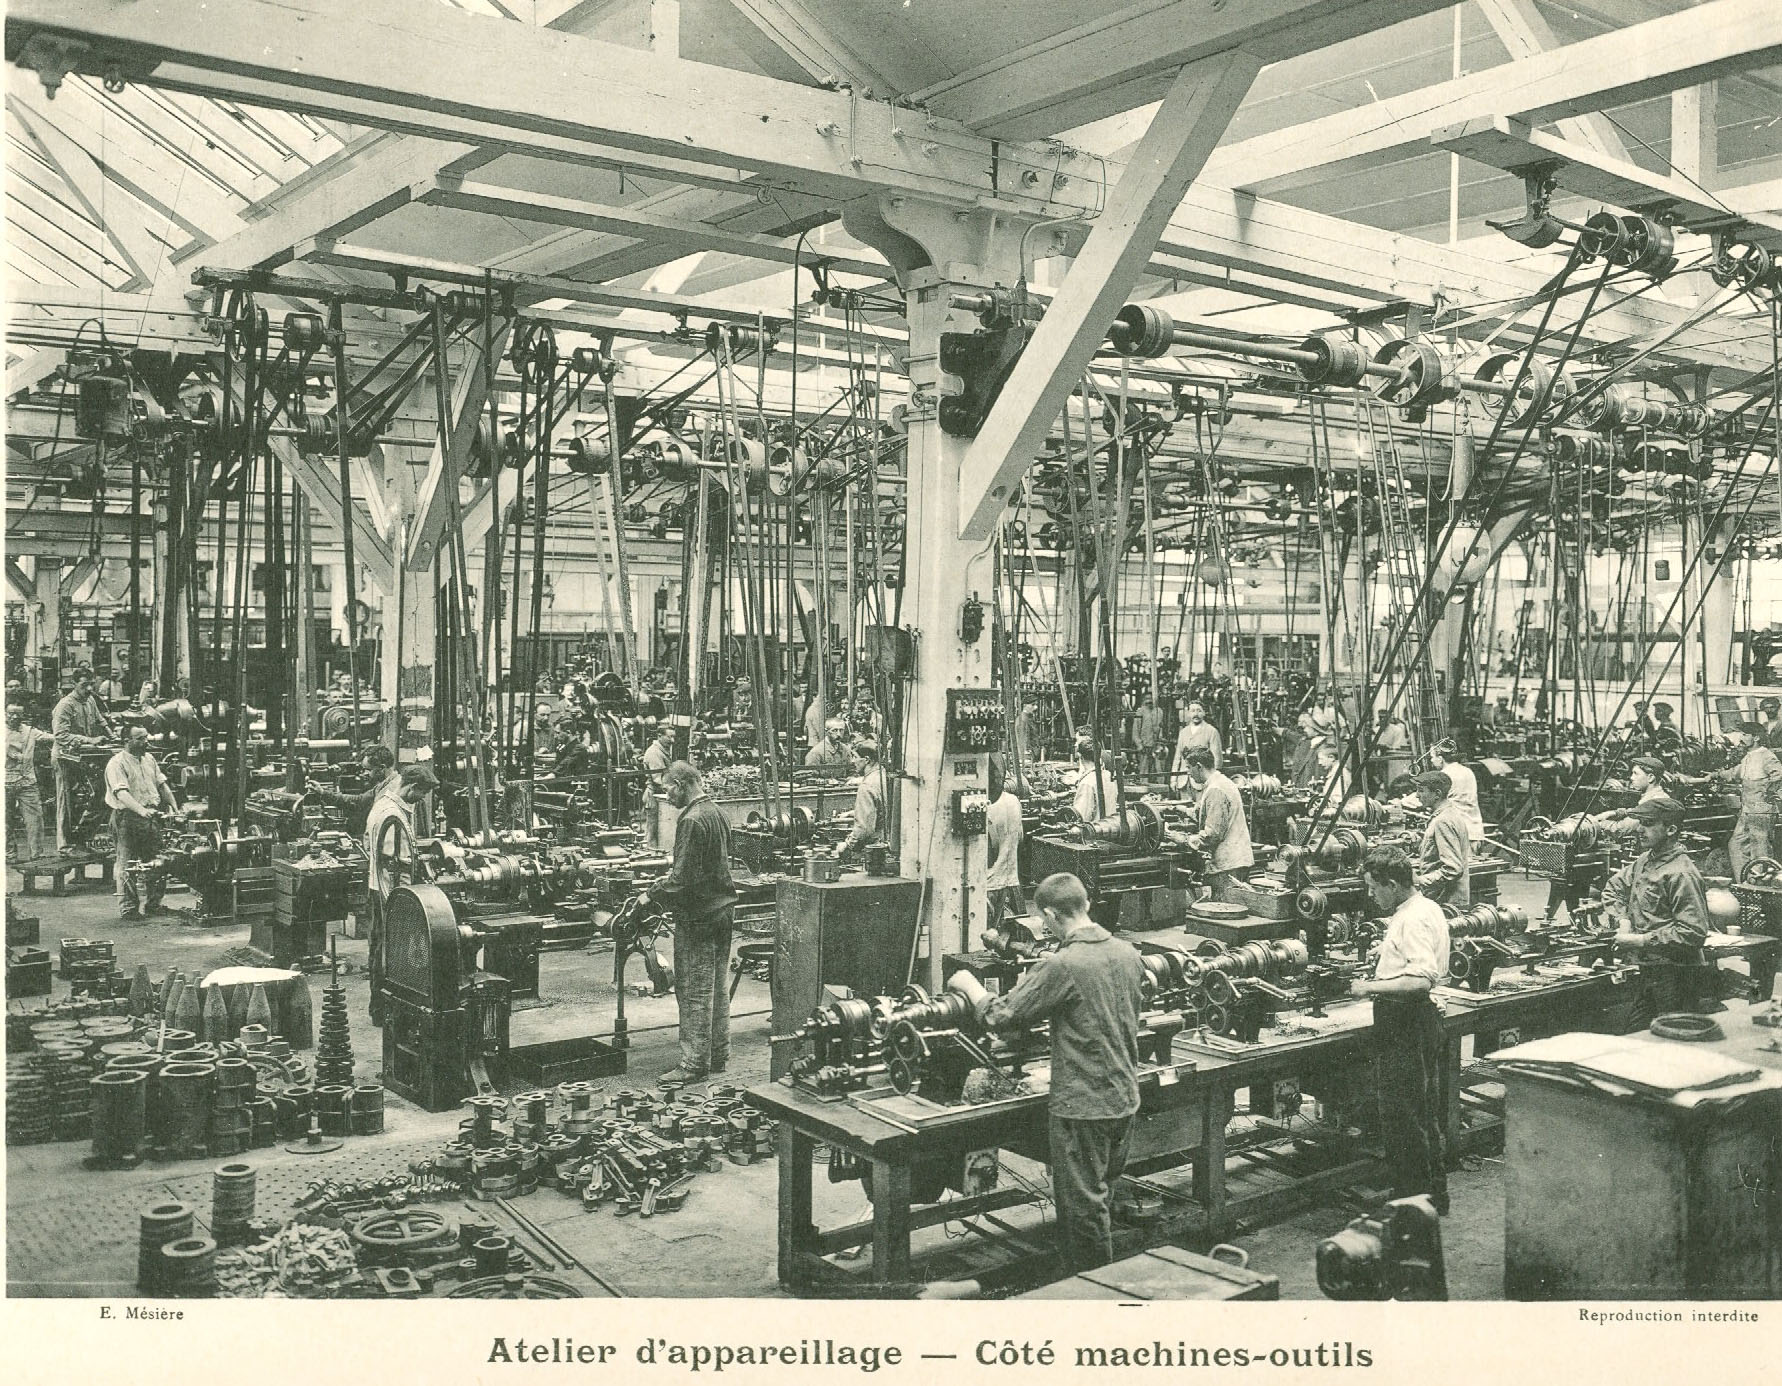
\includegraphics[width=1\textwidth]{assets/ontologie/Atelier d'appareillage - côté machines outils.jpg}
    \caption{Image utilisée afin de dresser le premier schéma expliquant les articulations entre les différentes ontologies}
    \label{fig:photoInspiSchemaBase}
\end{figure}

\paragraph{} \hspace{10mm}
L'ensemble de l'ontologie est centrée sur celle du \textbf{CIDOC-CRM}. Pour pouvoir suivre les normes de l'industrie, nous nous sommes fixés certaines règles à suivre qui permettent deux choses : premièrement, cela facilite l'alignement de notre ontologie avec celles des autres projets de \textbf{LabInVirtuo} et secondement, cela permet de garder une certaine normalisation de notre travail.

Dans l'absolu, CIDOC-CRM permet de faire presque tout ce dont on a besoin. Du moins, même si certaines classes et propriétés ne sont pas celles que l'on utilise le plus (car d'autres ontologies font mieux et sont par conséquent plus utilisées pour ces cas là), elles ont au moins le mérite d'exister et de nous permettre de combiner plusieurs ontologies facilement. Ainsi, voici la liste des règles fixées et modifications que nous avons apportées pour avoir un résultat qui répond à nos besoins :
\begin{itemize}
    \item[\ding{103}] CIDOC-CRM n'ayant pas de classes très précises pour décrire les documents et images que nous utilisons comme source d'information, nous avons utilisé \textbf{bibo} en remplacement. Ainsi, la classe \textbf{crm:E36 Visual Item} est déclarée équivalente à \textbf{bibo:Image} et \textbf{crm:E31 Document} est équivalent à \textbf{bibo:Document}\footnote{La déclaration d'une équivalence de classe se fait via l'ajout d'un triplet RDF dans la déclaration de l'ontologie de la manière suivante : \textit{bibo:Image owl:EquivalentClass crm:E36\_Visual\_Item ;}}. La classe \textbf{bibo:Document} ayant 21 classes filles décrivant des types de documents, cela nous permet d'être plus précis dans la saisie de nos données.
    \item[\ding{103}] Comme pour les images et documents, l'ontologie CIDOC-CRM manque de rigueur pour décrire les acteurs. Les deux classes existantes sont \textbf{crm:E21 Person} et \textbf{crm:E74 Group} mais leurs définitions dans la documentation ne permettent pas de bien faire la différence entre personne physique, personne morale et groupe de personnes physiques. Par conséquent, nous utilisons l'ontologie \textbf{RDA} qui possède plus de classes et de propriétés pour décrire les acteurs qu'ils soient physiques ou moraux et nous avons créé les équivalents suivants : \textbf{rdac:Person} avec \textbf{crm:E21 Person}, \textbf{rdac:Corporate Body} avec \textbf{crm:E74 Group} et \textbf{crm:E39 Actor} avec \textbf{rdac:Collective Agent}. Pour décrire une personne physique, nous utilisons \textbf{rdac:Person}, pour un groupe de personnes, nous utilisons \textbf{rdac:Corporate Body} et pour les personnes morales, nous employons \textbf{rdac:Collective Agent}. Nous utilisons aussi les propriétés de \textbf{RDA} pour décrire les acteurs plutôt que les propriétés \textbf{CIDOC-CRM}.
    \item[\ding{103}] En ce qui concerne \textbf{dcterms}, il a fallu ajouter un \textbf{domain}\footnote{Le "domain" d'une propriété est le type de classe sur lesquelles s'appliquent la-dite propriété. Autrement dit, c'est la classe du sujet du triplet RDF} aux différentes propriétés qui n'en avaient pas. En théorie, le fait qu'une propriété n'ait pas de domain n'est pas vraiment gênant car cela autorise une certaine liberté quant à son utilisation, mais dans notre cas nous n'avons aucun intérêt à le faire puisque l'on sait comment va être exploitée l'ontologie. En conséquence, nous avons choisi \textbf{bibo:Document} comme range (pour les propriétés pour lesquelles c'est pertinent et que nous utilisons) : tous les types de documents sont couverts, images incluses, étant donné que \textbf{bibo:Image} hérite de \textbf{bibo:document}. Pour les propriétés que nous n'utilisons pas, nous avons choisi \textbf{owl:Thing} pour ne pas laisser le domain vide. Pour toutes les propriétés que nous utilisons, le domain choisi reste pertinent.
    \item[\ding{103}] Pour l'ontologie \textbf{schema}, deux choix se sont proposés à nous : nous pouvions soit modifier le domain et la range\footnote{Comme pour le domain, la range est équivalente à l'objet d'un triplet} des propriétés et garder uniquement les propriétés dans notre ontologie, soit garder les mêmes domain et range, et de ce fait garder les classes nécessaires pour ensuite créer des équivalences de classe. Pour des raisons de praticité, nous avons opté pour la deuxième option car dans le cas où nous aurions eu le besoin d'utiliser de nouvelles propriétés de cette ontologie, nous n'aurions pas eu à modifier chaque propriété une par une. Les équivalences de classes sont donc : \textbf{schema:Person} avec \textbf{rdac:Person} et \textbf{schema:Place} avec \textbf{crm:E53 Place}.
    \item[\ding{103}] Enfin, nous avons procédé exactement de la même manière pour \textbf{relationship}. L'ontologie utilisant \textbf{foaf:Person} pour ses domain et range, nous avons déclaré que \textbf{foaf:Person} était équivalente à \textbf{rdac:Person}.
\end{itemize}

\paragraph{} \hspace{10mm}
Cependant, nous n'avons pas gardé toutes les classes et propriétés des ontologies dans la déclaration de la nôtre. En effet, nous avons supprimé une majeure partie de \textbf{schema} car elle ne nous servait pas. La raison qui nous a poussé à faire ce choix est que l'ontologie \textbf{schema} est très dense et contient beaucoup de classes et propriétés, ce qui signifie que sa déclaration est très longue. Nous avons donc préféré supprimer le contenu inutilisé pour que notre déclaration de l'ontologie TTM ne le soit pas elle aussi, d'autant plus que \textbf{schema} a été choisie pour seulement deux propriétés en particulier. En revanche, nous n'avons pas supprimé toutes les propriétés inutiles de \textbf{RDA}. L'ontologie nous étant utile pour un plus grand nombre de propriétés et n'étant probablement pas exploitée à 100\% des besoins que nous pourrions avoir, il aurait fallu vérifier les 1100 propriétés une par une à la main pour savoir lesquelles nous pourrions garder et lesquelles pourraient être supprimées sans soucis.

\paragraph{} \hspace{10mm}
En vue de pouvoir établir la déclaration de notre ontologie, nous nous sommes aidés de deux outils : la bibliothèque python \href{https://rdflib.readthedocs.io/en/stable/}{\textbf{RDFLib}} et le logiciel \textbf{Protégé}. Les deux sont plutôt complémentaires malgré le fait qu'ils n'aient pas été développés dans ce but, le premier permettant de facilement modifier une grande quantité de triplets et le second permettant de rendre plus visuelles les ontologies, facilitant ainsi des petites modifications ciblées. Pour montrer un exemple de l'utilité de \textbf{RDFLib}, on peut citer par exemple la modification de toutes les propriétés de \textbf{RDA} : par défaut, la plupart des propriétés de RDA sont de type \textbf{owl:AnnotationProperty}\footnote{Il existe trois types de propriétés : les \textbf{owl:DatatypeProperty} qui prennent pour valeur des valeurs littérales (nombres, dates, chaînes de caractères, etc), les \textbf{owl:ObjectProperty} qui prennent pour valeur des objets et les \textbf{owl:AnnotationProperty} qui prennent pour valeur soit des valeurs littérales soit des objets.}, ce que nous ne souhaitons pas car ces propriétés sont non-logiques (elles sont ignorées lors de la validation, donc on ne peut pas savoir si elles enfreignent les règles logiques). Par conséquent, en seulement quelques lignes de code nous avons pu remplacer leur type, passant de \textbf{owl:AnnotationProperty} à \textbf{owl:ObjectProperty}, les propriétés d'annotation de l'ontologie s'appliquant de manière pertinente presque toujours sur des objets. Sans la bibliothèque, nous aurions dû vérifier chaque propriété à la main, tâche complètement impossible au vu de leur nombre.

\begin{figure} [H]
    \centering
    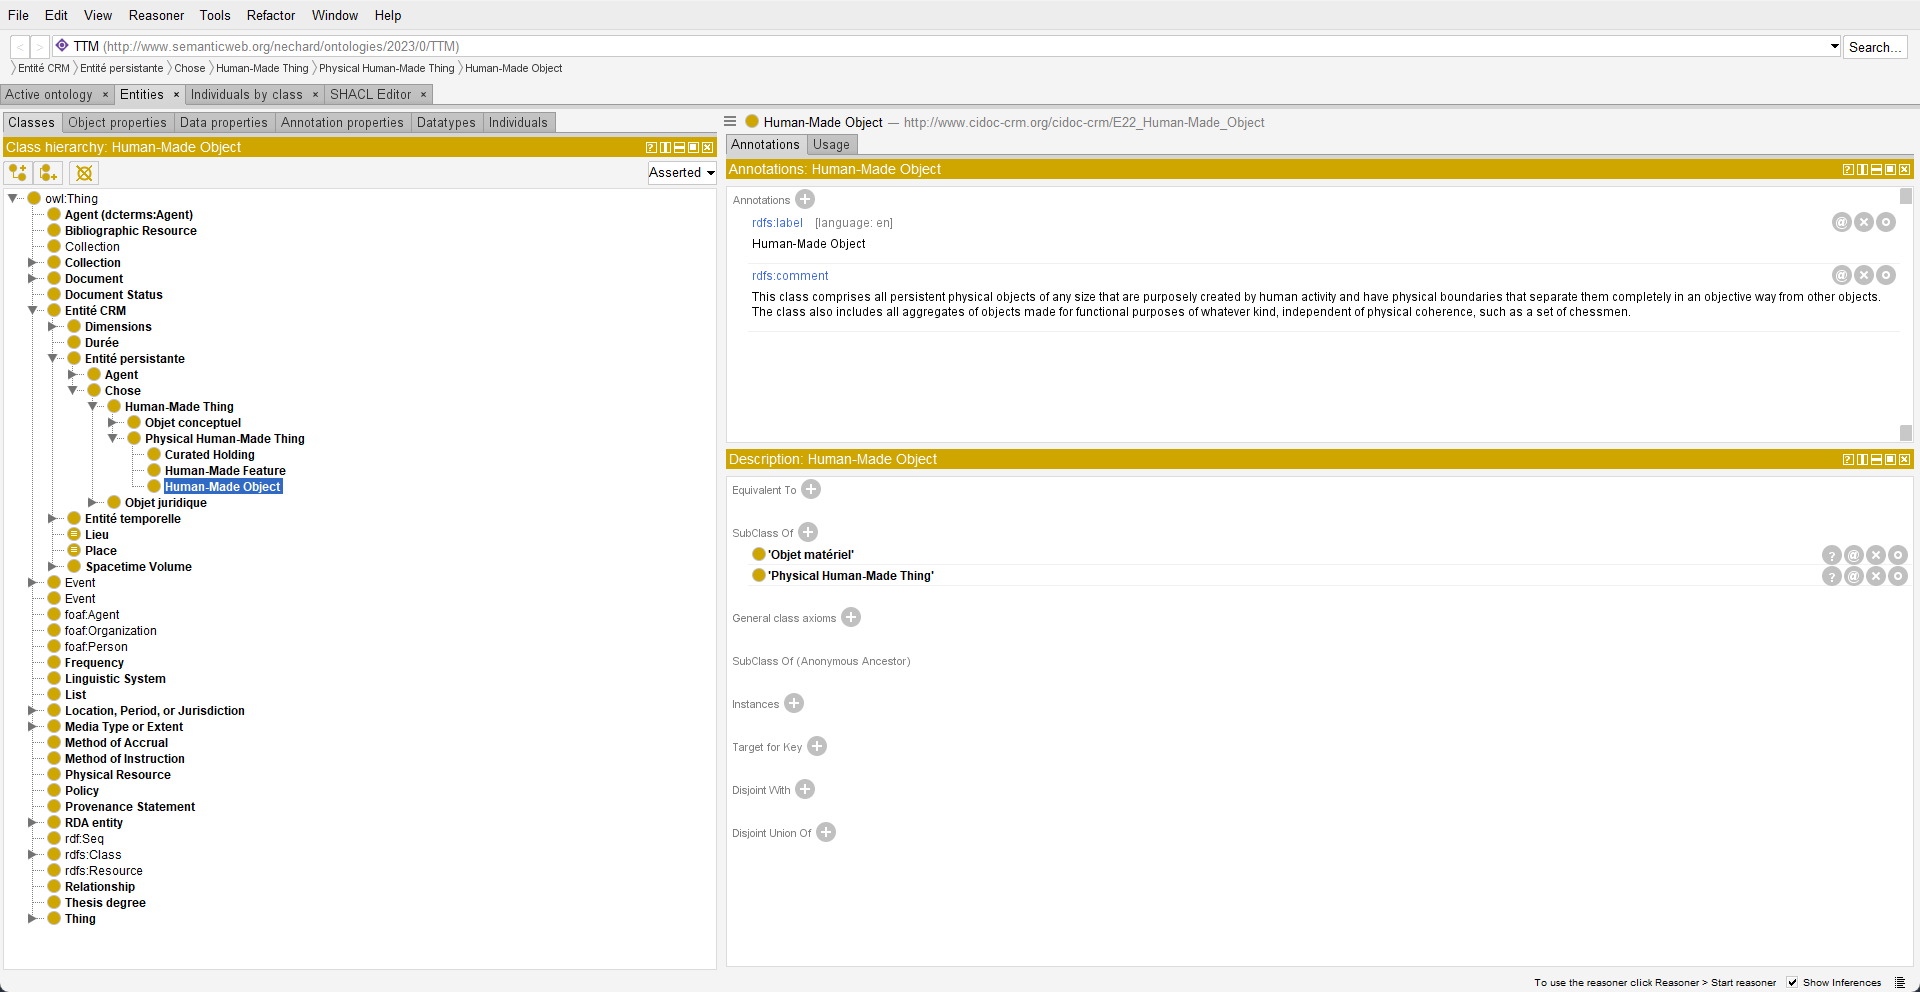
\includegraphics[width=1\textwidth]{assets/ontologie/Protege/screen_exemple_protege.png}
    \caption{Capture d'écran montrant l'interface de Protégé (visualisation de la classe \textbf{crm:E22 Human-Made Object})}
    \label{fig:screenExempleProtege}
\end{figure}

\subsubsection{Le cas spécial des flux}

\paragraph{} \hspace{10mm}
Une des difficultés auxquelles nous avons dû faire face avec Cyril et Matthieu est la modélisation des flux. De base \textbf{CIDOC-CRM} ne dispose pas de classe spécialement dédiée. Nous avons donc eu le choix entre deux options : trouver une nouvelle ontologie à intégrer à la nôtre ou bien tenter d'utiliser la classe \textbf{crm:E9 Move} du CIDOC-CRM malgré le nombre restreint de propriétés existantes dû au fait que CIDOC-CRM n'a pas été pensée pour ça. Pour des raisons de praticité (i.e. limiter au maximum le nombre d'ontologies que nous utilisons), nous avons opté pour la deuxième option. Au moment où nous avons fait ce choix, nous ne savions pas si il pourrait être concluant, Matthieu Quantin n'ayant jamais été confronté à cette situation auparavant.

\paragraph{} \hspace{10mm}
Pour pouvoir modéliser les flux de la manière la plus simple possible, nous avons scindé le problème en sous-problèmes : 
\begin{itemize}
    \item[\ding{103}] comment lier le flux à ce qui a été déplacé ?
    \item[\ding{103}] comment lier le flux à la durée du déplacement ?
    \item[\ding{103}] comment lier le flux au lieu de départ et au lieu d'arrivée ?
    \item[\ding{103}] comment faire si le flux peut (ou doit) être divisé en sous-flux ?
\end{itemize}

\paragraph{} \hspace{10mm}
Au final, nous avons réussi assez rapidement à résoudre ces sous-problèmes en fouillant dans la documentation. CIDOC-CRM possède précisément les bonnes propriétés dont nous avons eu besoin, et sont au nombre de 5 pour les plus utiles : 
\begin{itemize}
    \item[\ding{103}] \textbf{crm:P25 Moved} permet de modéliser ce qui a été déplacé. La range de la propriété est un \textbf{crm:P19 Physical Object}.
    \item[\ding{103}] \textbf{crm:P191 had duration} permet d'indiquer le temps de déplacement du point de vue quantitatif (valeur numérique) et dimensionnelle.
    \item[\ding{103}] \textbf{crm:P26 Moved to} et \textbf{crm:P27 Moved from} permettent de modéliser le point de départ et d'arrivée du flux. Ils doivent être des endroits physiques car la range de la propriété est \textbf{crm:P53 Place} (il faut donc utiliser d'autres propriétés pour un transfert d'argent d'un compte bancaire à un autre par exemple).
    \item[\ding{103}] \textbf{crm:P9 Consists of} permet de découper un flux en sous-flux. C'est donc une propriété symétrique dont le domaine et la range sont \textbf{crm:E9 Move}.
\end{itemize}

\begin{figure} [H]
    \centering
    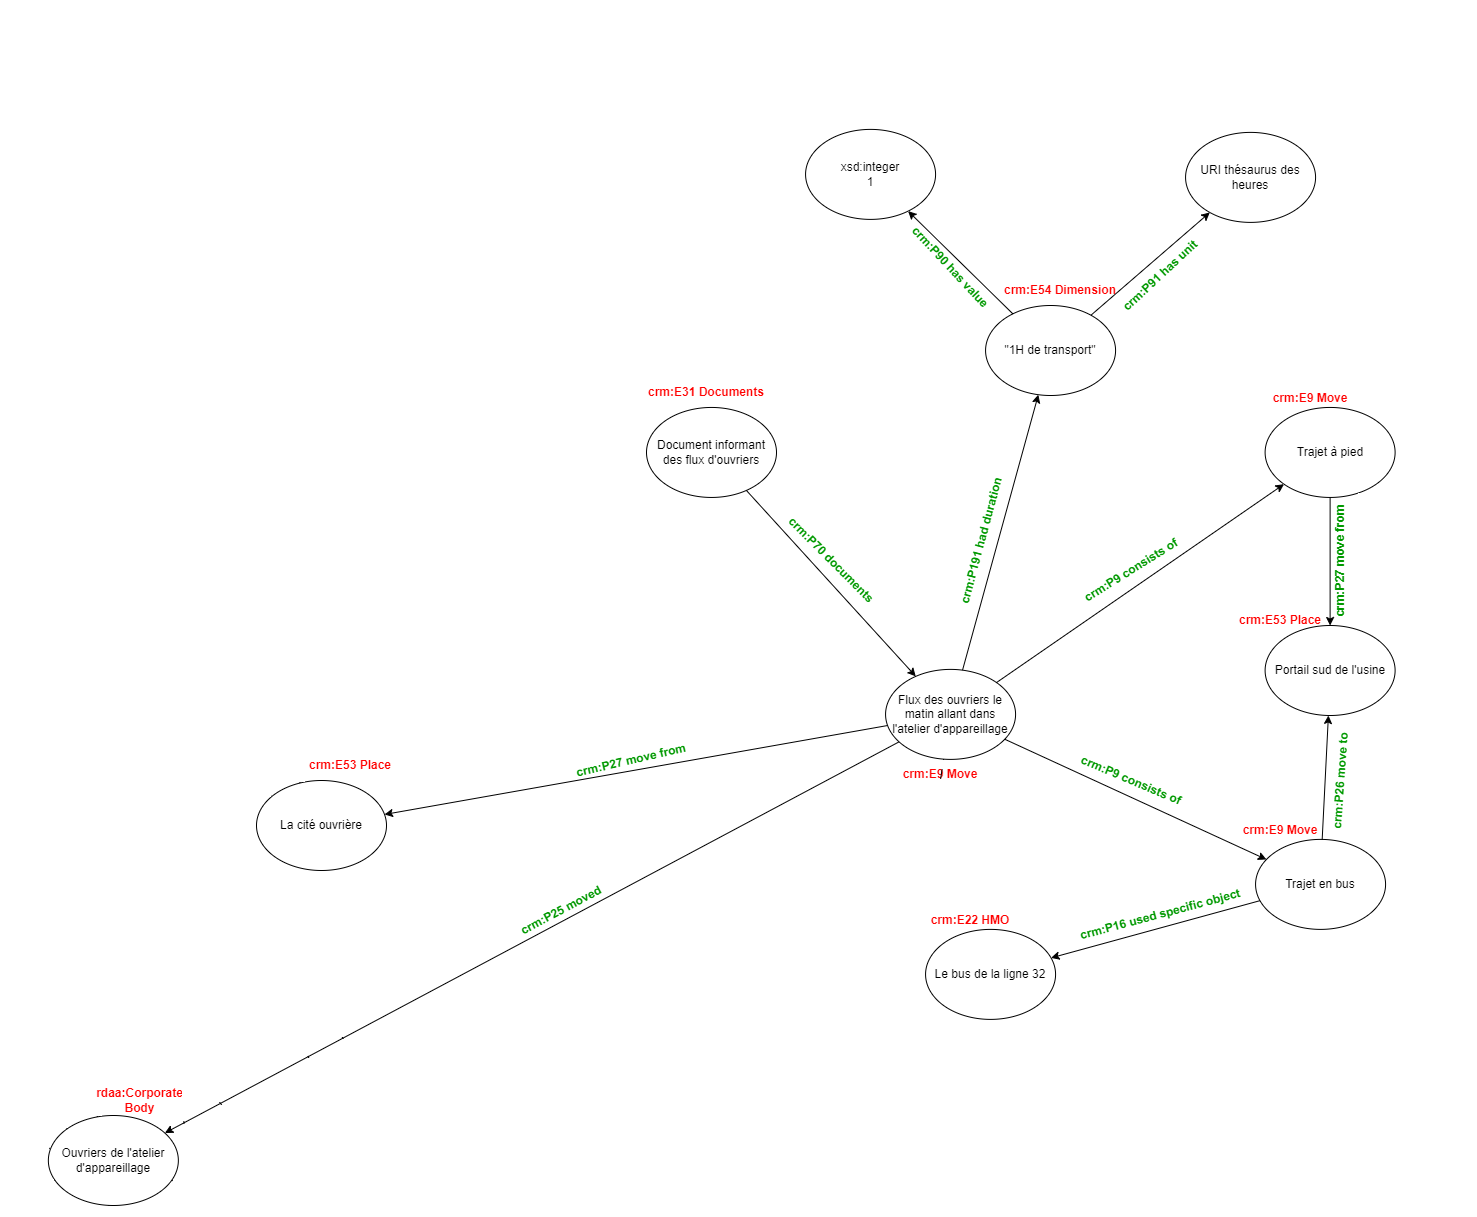
\includegraphics[width=1\textwidth]{assets/ontologie/screen_flux.png}
    \caption{Schéma montrant la modélisation des flux (extrait du schema général)}
    \label{fig:screenFlux}
\end{figure}

\subsection{Omeka-S et saisie des données}

\paragraph{} \hspace{10mm}
Pour créer la nouvelle base de données basée sur un modèle ontologique, deux choix ce sont présentés à nous : \textbf{Omeka-S} ou un système de \textbf{triple-store}. Malgré la capacité du triple-store à stocker une très grande quantité de données, nous avons choisi d'utiliser Omeka-S pour plusieurs raisons : 
\begin{itemize}
    \item[\ding{103}] tout d'abord, Omeka-S est bien plus simple à mettre en place et à utiliser qu'un triple-store.
    \item[\ding{103}] ensuite, le fait que l'ancienne base du projet ne contenait pas de données a beaucoup influencé notre choix. Si l'ancienne base avait déjà été remplie, il aurait fallu "transvaser" les données d'une base à l'autre ce qui aurait nécessité de créer un outil spécial pour convertir le format des données, d'autant plus  qu'il est beaucoup plus simple de transférer ces données vers un triple-store que vers Omeka-S. Par conséquent, dans le cas où l'ancienne base aurait été remplie, il aurait été pertinent d'utiliser un triple-store mais puisque ce n'est pas le cas, Omeka-S reste une bonne option.
    \item[\ding{103}] enfin, les compétences et connaissances de Matthieu Quantin sur Omeka-S, ainsi que le fait qu'il n'ait jamais mis en place de triple-store ont entériné notre choix.
\end{itemize}

\begin{figure} [H]
    \centering
    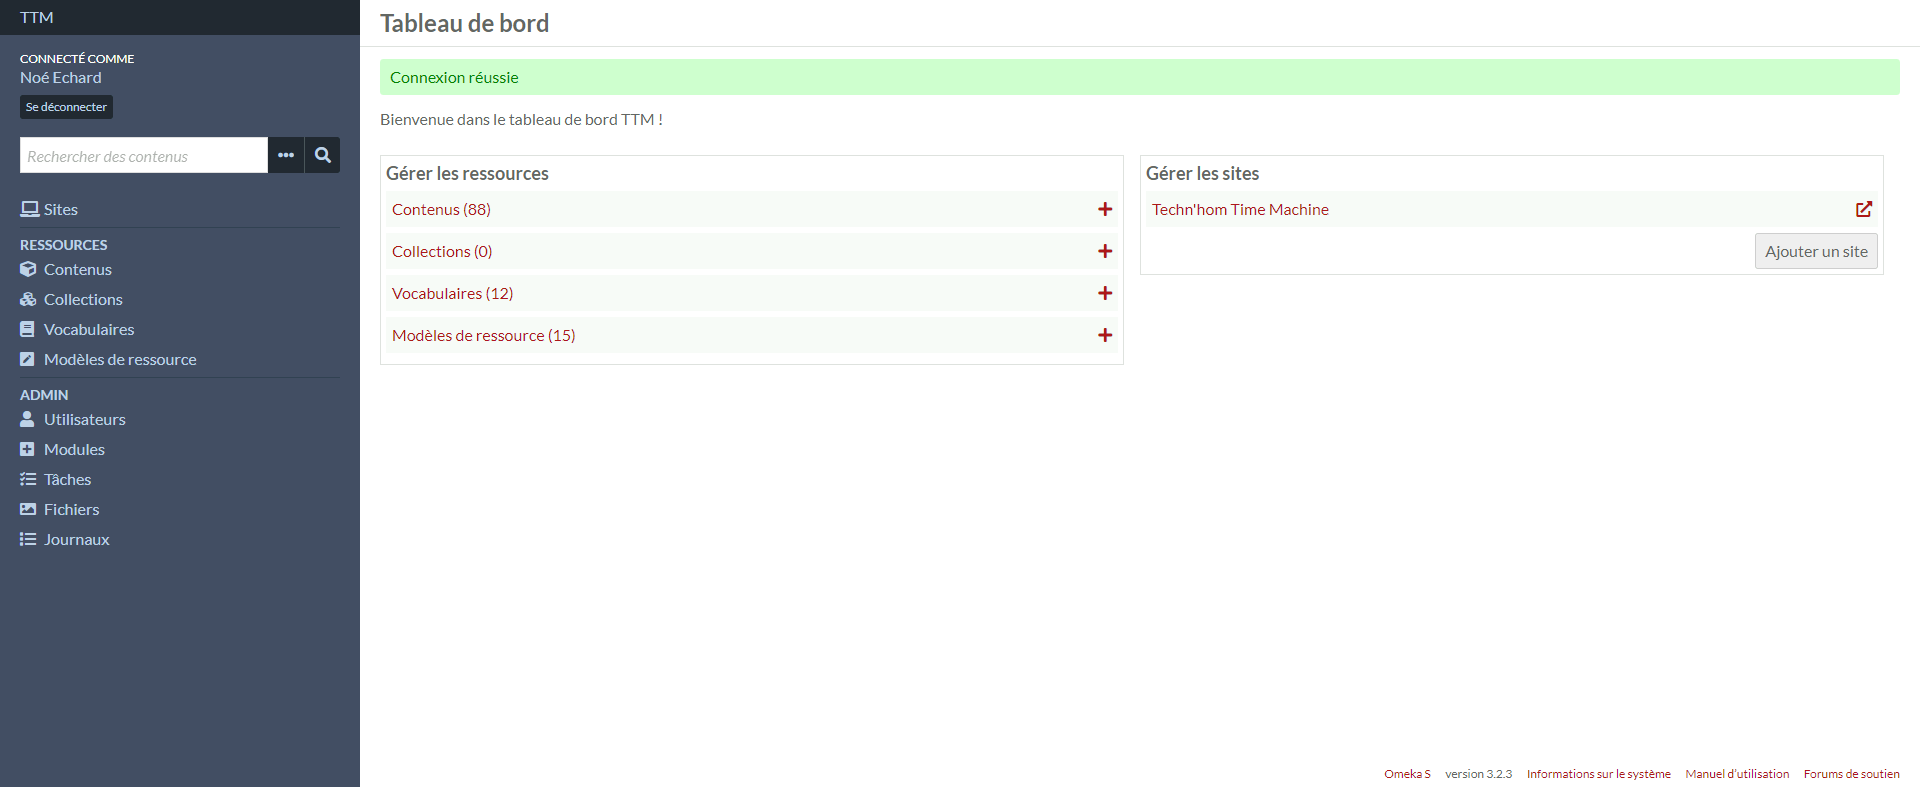
\includegraphics[width=1\textwidth]{assets/omeka/panneau_admin_omekapng.png}
    \caption{Écran d'accueil du panneau administrateur d'Omeka-S}
    \label{fig:panneauAdminOmeka}
\end{figure}

\subsubsection{Mise en place d'Omeka}

\paragraph{} \hspace{10mm}
L'un des principaux avantages d'Omeka-S est son aspect "clé en main". Malgré la rigidité qu'une telle caractéristique impose, Omeka-S reste assez ouvert au niveau de la personnalisation et du paramétrage. C'est donc la première tâche à laquelle nous nous sommes attelés avant de commencer à saisir les données. 

\paragraph{} \hspace{10mm}
Parmi tout ce que nous avons eu à faire, nous avons tout d'abord commencé par créer toutes les pages (autres que celle qui affiche les données) visibles sur le site web. Parmi ce qui avait été fait par Gabriel et Guillaume, nous avons repris les pages présentant le projet et l'équipe de travail et nous avons créé deux pages, nommées assez logiquement "Projet" et "Equipe" (voir Annexe 3, \hyperref[fig:pageProjetOmeka]{figure 3.16} et \hyperref[fig:pageEquipeOmeka]{figure 3.17}).

Ensuite, nous avons installé des thèmes et extensions. Parmi tous les thèmes disponibles, nous en avons pris quelques-uns qui nous semblaient convenir pour le projet afin de les tester. Au final, nous avons selectionné le thème "Center Row". Nous avons également installé des extensions, notamment celle nommé "Log" et qui permet d'avoir tous les logs des erreurs ou warnings directement dans le panneau d'admin via un onglet dédié.

\begin{figure} [H]
    \centering
    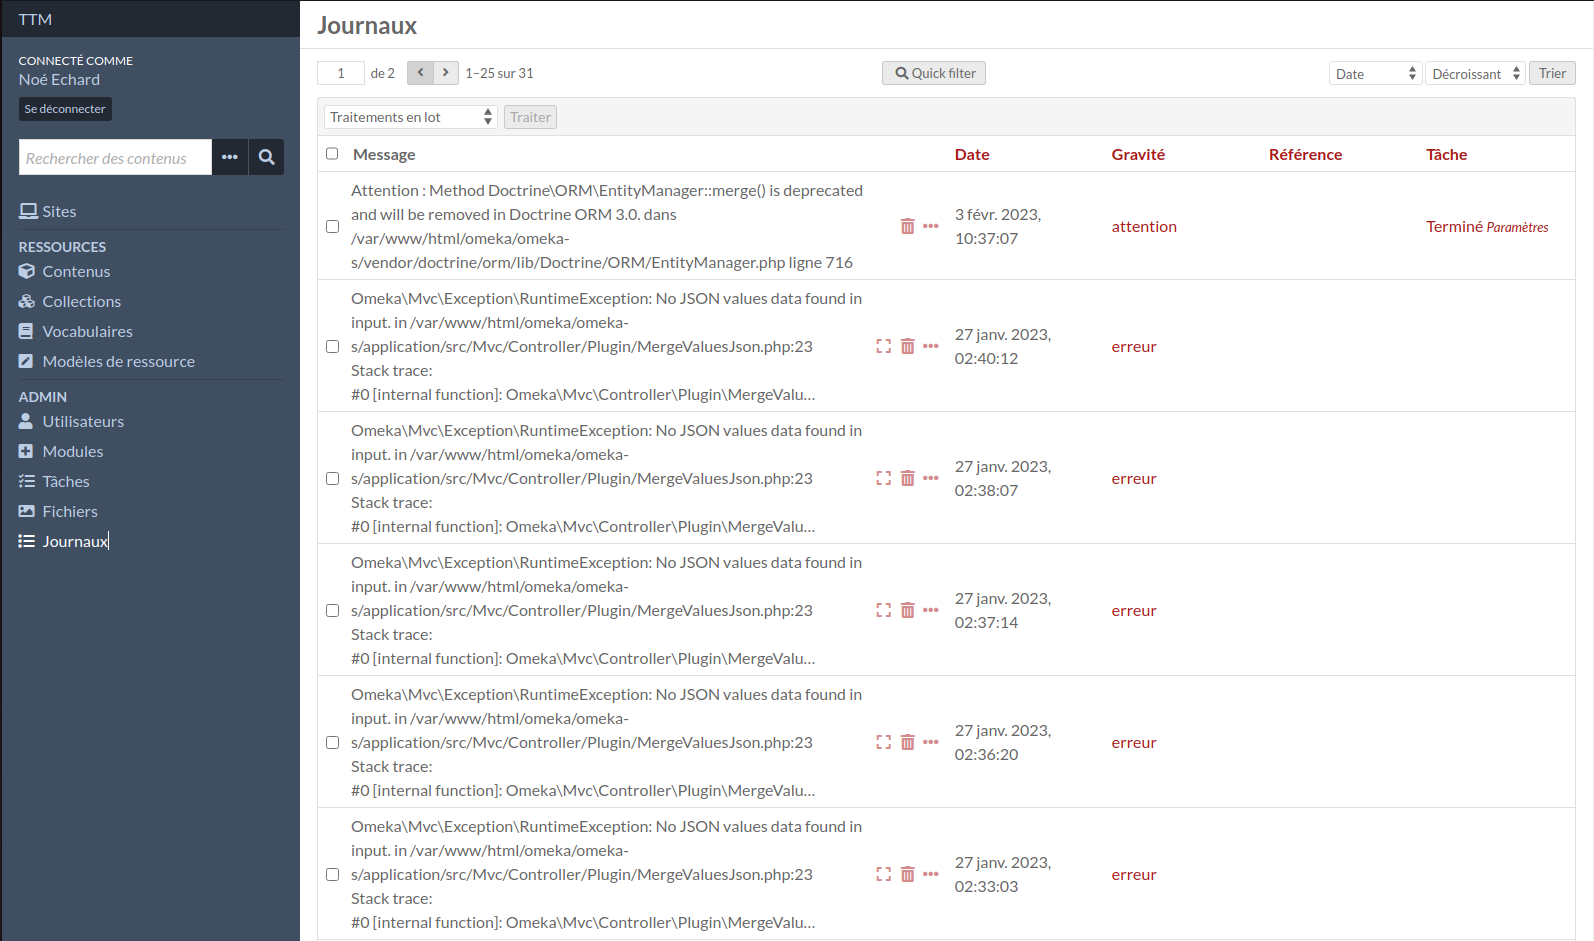
\includegraphics[width=1\textwidth]{assets/omeka/onglet_logs_omeka.png}
    \caption{Onglet des logs d'Omeka-S}
    \label{fig:ongletLogsOmeka}
\end{figure}

\subsubsection{Saisie des données}

\paragraph{} \hspace{10mm}
Une fois la "mise en place globale" terminée, nous nous sommes occupés de celle pour les ontologies et la saisie des données. La première étape a été de charger tous les vocabulaires\footnote{Comprendre ontologie} nécessaires à la saisies des données. Certains sont présents de base (comme \textbf{owl} ou \textbf{rdf} par exemple) mais la plupart doivent être chargés à l'aide du fichier contenant la déclaration de l'ontologie et du namespace\footnote{URL où se trouve le code de la déclaration sur internet}.

\begin{figure} [H]
    \centering
    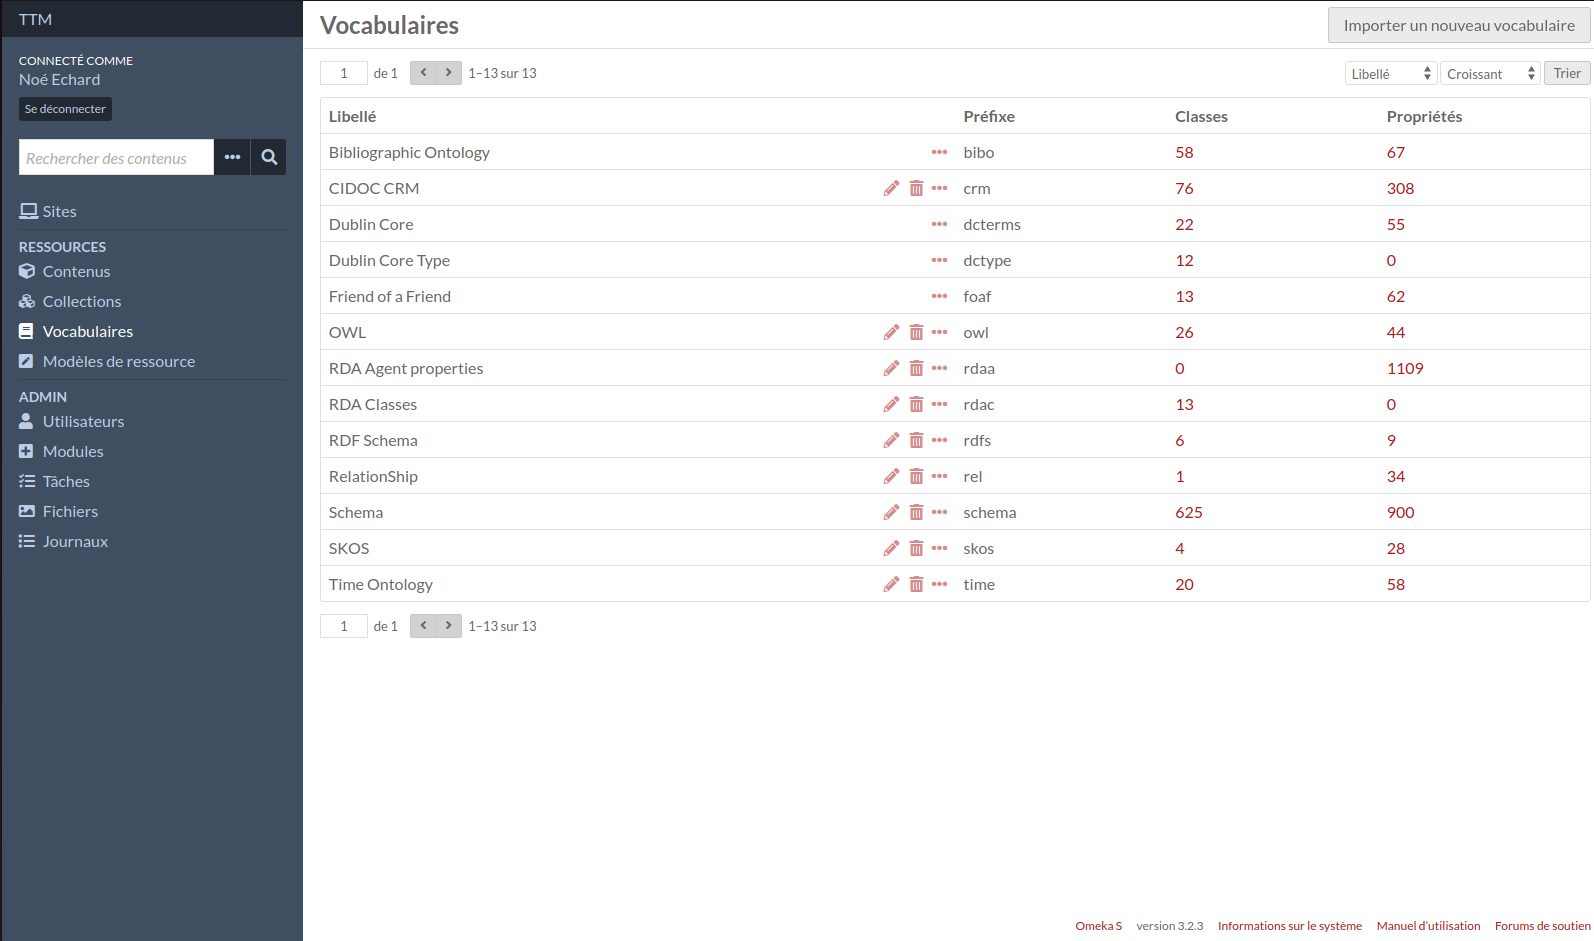
\includegraphics[width=0.82\textwidth]{assets/omeka/onglet_vocabs_omeka.png}
    \caption{Onglet des vocabulaires chargés dans Omeka-S}
    \label{fig:ongletVocabsOmeka}
\end{figure}

\paragraph{} \hspace{10mm}
Une fois les vocabulaires chargés, il ne manque plus qu'une étape avant de pouvoir saisir les données : créer des modèles de ressources. Même s'ils ne sont techniquement pas obligatoires, leur utilisation est presque requise tant le gain de temps est grand lorsque l'on enregistre des données. D'autant plus qu'ils permettent d'imposer certaines règles à ceux qui les utilisent.

De fait, tous les modèles de données que nous avons créés possèdent plusieurs caractéristiques :
\begin{itemize}
    \item[\ding{103}] La ressource créée a toujours un champ \textbf{skos:prefLabel} quelle que soit sa classe, et sa saisie est obligatoire.
    \item[\ding{103}] Le champ \textbf{skos:prefLabel} est affiché en tant que titre de ressource (par défaut le titre est de type \textbf{dcterms:title}).
    \item[\ding{103}] Toutes les propriétés ont un nom d'affichage renommé. Cela permet d'avoir un nom français, propre et lisible sur le site (par exemple, "hasDateOfBirth" devient "Date de naissance"). De surcroît, toutes les propriétés utilisées pour enregistrer un item qui ne sont pas dans le modèle de ressource ne peuvent pas être renommées pour l'affichage du site.
\end{itemize}

\begin{figure} [H]
    \centering
    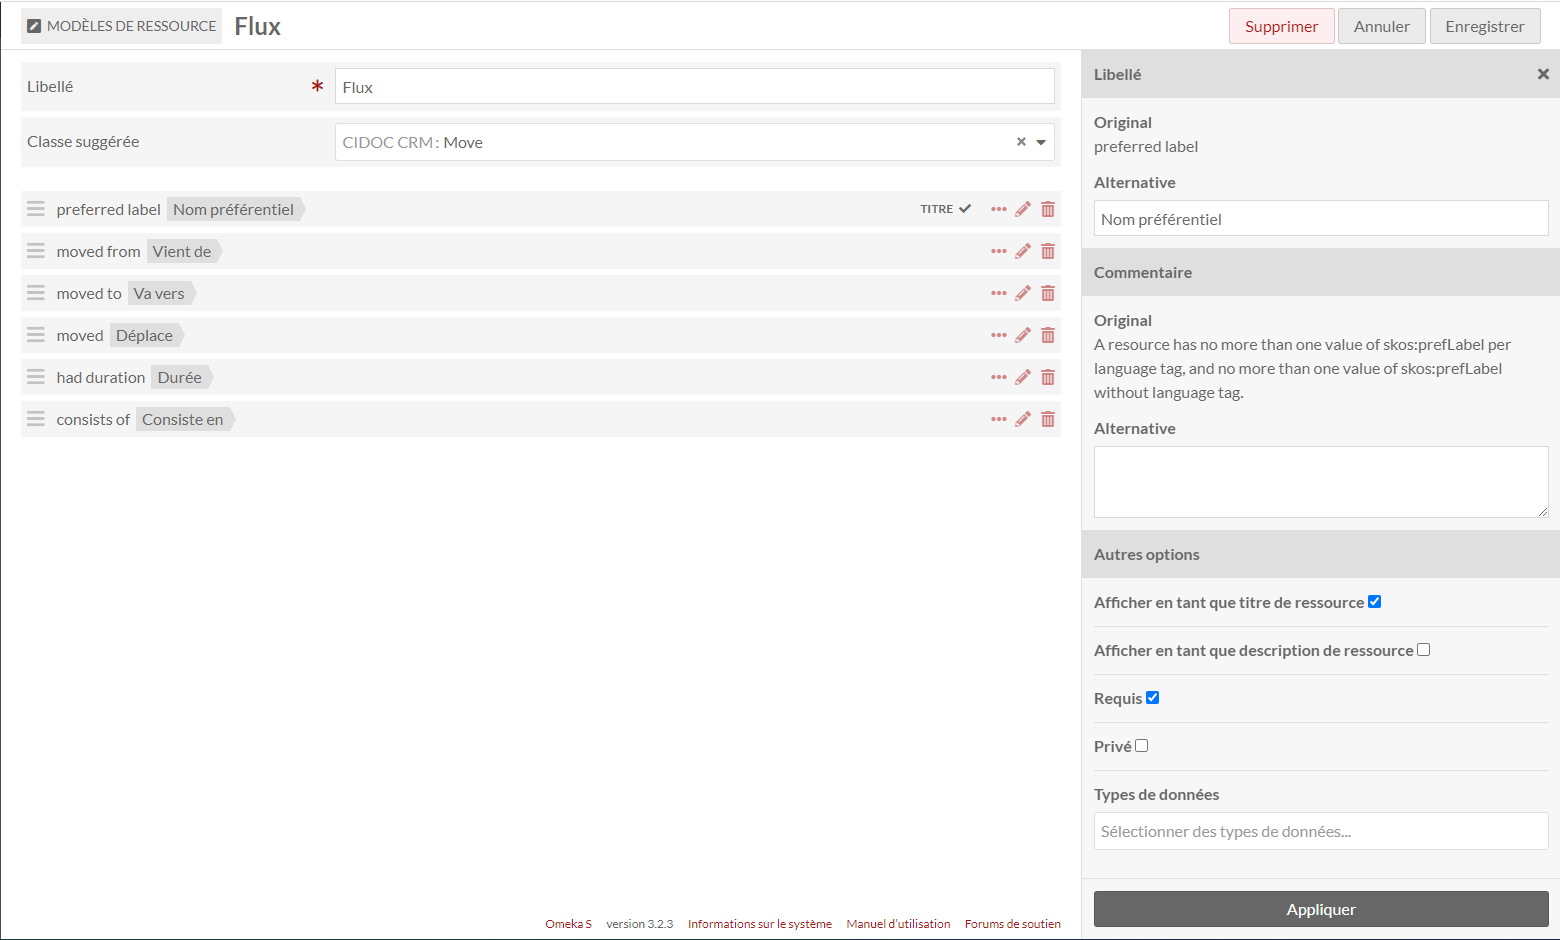
\includegraphics[width=1\textwidth]{assets/omeka/screen_omeka_modele_ressource.png}
    \caption{Exemple de modèle de ressource en cours d'édition}
    \label{fig:modeleRessourceOmeka}
\end{figure}

\paragraph{} \hspace{10mm}
Après avoir terminé la préparation, nous avons enfin pu commencer à saisir des données. Les premiers items que nous avons documentés sont tous tirés du manuel Roret intitulé "Nouveau manuel complet du filateur". Cyril s'est chargé de son analyse, puis a synthétisé toutes les informations utiles dans un document Word à l'aide de tableaux et de petits textes explicatifs. A partir de son document d'analyse, nous avons pu dresser dans un premier temps le schéma décrivant la production de coton (\hyperref[fig:schemaRoretTTM]{figure 3.17}), et c'est seulement dans un second temps que nous avons saisi les données.

\begin{figure} [H]
    \centering
    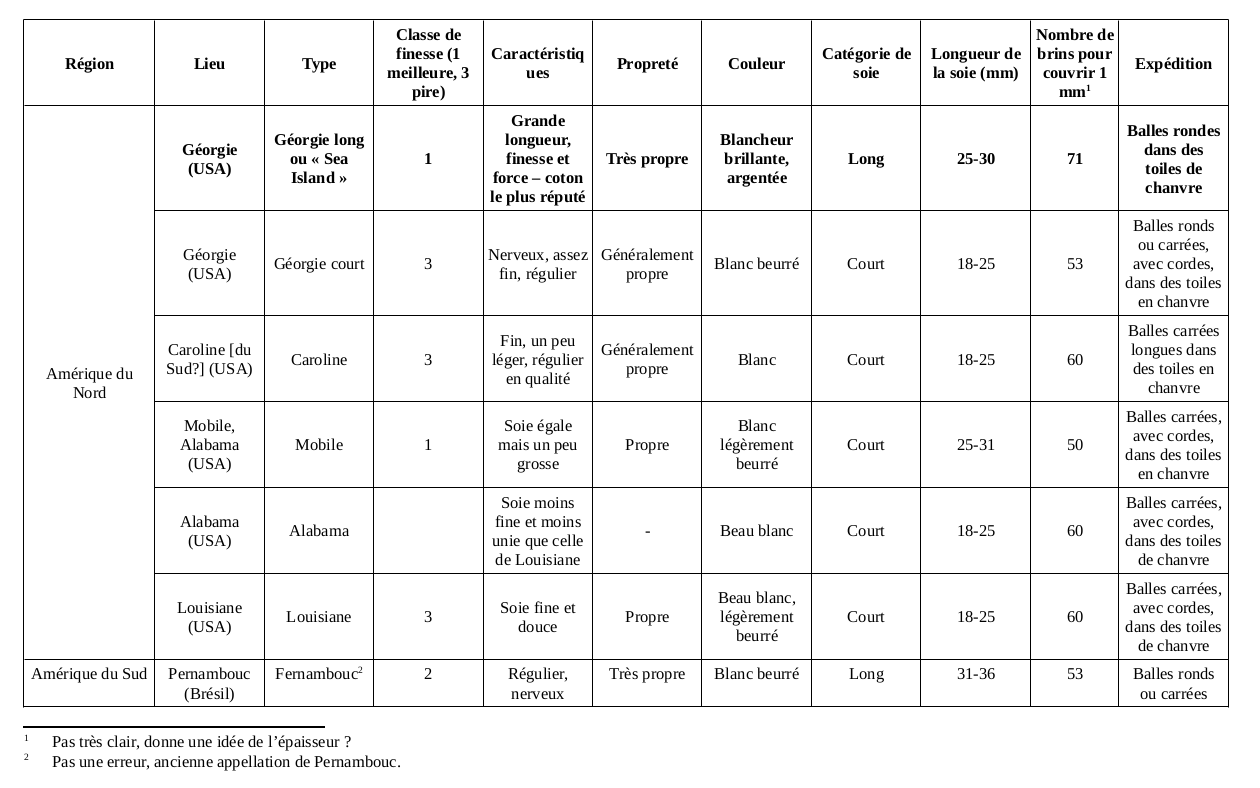
\includegraphics[width=1\textwidth]{assets/divers/screen_cotons.png}
    \caption{Exemple de tableau récapitulant les informations à enregistrer pour certains types de cotons}
    \label{fig:screenTableauCoton}
\end{figure}

\subsection{Thésaurus}

\paragraph{} \hspace{10mm}
L'un des aspects essentiels de l'utilisation d'ontologies sont les thésaurus documentaires. Ils permettent de lier des items non normalisés et non contrôlés à des listes de termes qui eux, le sont. L'utilisation de thésaurus est primordiale, car elle permet de faciliter les alignements entre différentes ontologies, fondement essentiel à leur existence même.

Dans le cadre de notre projet, et dans la volonté de suivre les normes de l'industrie, nous avons utilisé les ontologies suivantes :
\begin{itemize}
    \item[\ding{103}] \href{https://viaf.org/}{VIAF}, pour les personnes (ne fonctionne que si elles sont connues).
    \item[\ding{103}] \href{https://sws.geonames.org/}{GeoNames}\footnote{attention, l'URL est sws.geonames.org et non pas www.geonames.org}, pour les lieux
    \item[\ding{103}] \href{https://www.getty.edu/research/tools/vocabularies/aat}{Art and Architecture Thésaurus du Getty Museum}, pour toute notion autre qu'une personne ou un lieu
    \item[\ding{103}] \href{http://data.culture.fr/thesaurus/}{Les vocabulaires du Ministère de la Culture et de la Communication}, ici aussi pour toute notion autre qu'une personne ou un lieu (à la condition bien sûr, que le thésaurus détienne cette notion)
\end{itemize}

\paragraph{} \hspace{10mm}
Pour qu'un item soit lié à un thésaurus, nous devons utiliser la propriété \textbf{owl:sameAs}. De plus, bien que ces thésaurus possèdent l'essentiel des notions dont nous pourrions avoir besoin, nous avons aussi à disposition l'Opentheso\footnote{Opentheso est un logiciel de stockage de thésaurus en ligne} du projet "Huma-Num". Celui-ci regroupe toutes sortes de thésaurus portant sur des notions de Sciences Humaines et Sociales, le patrimoine industriel étant l'une d'entre elles. De plus, il regroupe tous les vocabulaires du Ministère de la Culture (nommé ci-avant) et permet de les parcourir via un arbre conceptuel, ce qui est plus rapide que de parcourir une par une les pages du site du ministère (sans parler du fait que le site du ministère est terriblement lent).  

\begin{figure} [H]
    \centering
    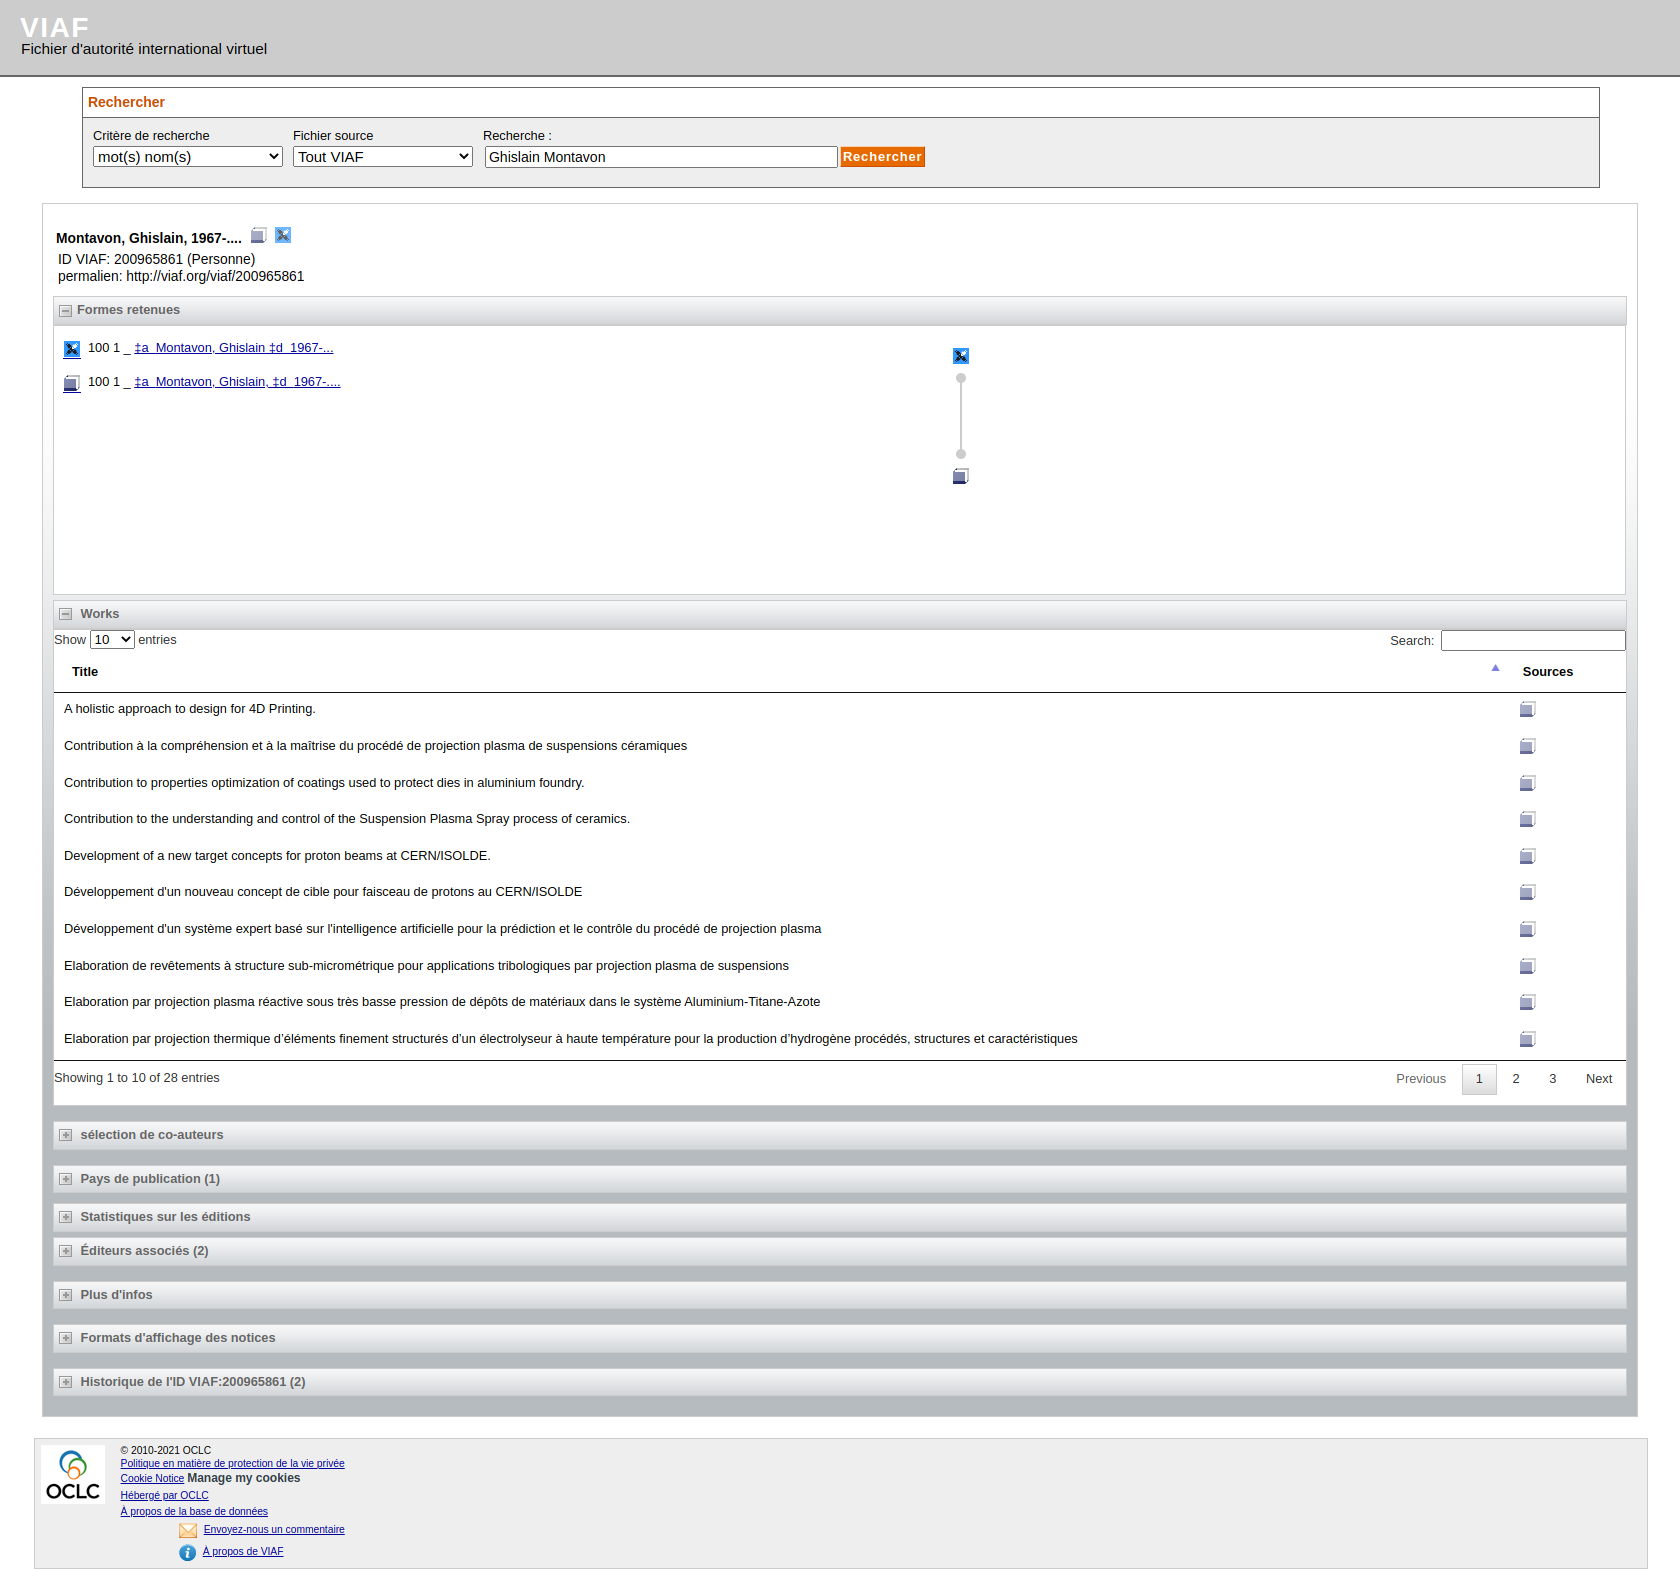
\includegraphics[width=1\textwidth]{assets/thesaurus/screen_viaf_ghis.png}
    \caption{Fiche VIAF de M. Ghislain Montavon}
    \label{fig:viafGhis}
\end{figure}

\subsection{Validation et SHACL}

\paragraph{} \hspace{10mm}
Avant que tout ce qui concerne la déclaration de notre ontologie et la saisie des données ne soit réellement terminé, il reste une étape cruciale à réaliser : la validation via la spécification SHACL (Shapes Constraints Language). Cette validation a deux intérêts majeurs :
\begin{itemize}
    \item[\ding{103}] s'assurer que les données saisies respectent bien les règles de notre ontologie (donc cela permet de corriger les erreurs).
    \item[\ding{103}] vérifier que notre ontologie en elle-même ne brise pas de règles logiques ou qu'il n'y ait pas d'incohérences.
\end{itemize}

\vspace{10mm}
Pour pouvoir mettre en place la validation, nous nous sommes aidés de deux outils :
\begin{itemize}
    \item[\ding{103}] Protégé et son plugin \textbf{SHACL4Protégé}
    \item[\ding{103}] l'outil de conversion de SPARNA : \hyperlink{https://shacl-play.sparna.fr/play/convert}{SHACL Play ! Convert}
\end{itemize}

\paragraph{} \hspace{10mm}
Ces deux outils ne peuvent fonctionner l'un sans l'autre : tout d'abord, à l'aide de "SPARNA Play !" et de notre fichier contenant notre ontologie, on génère un fichier SHACL qui va nous permettre de tester la validité de notre travail. Ensuite, à l'aide de Protégé, on charge le fichier SHACL puis on l'applique sur le fichier OWL contenant nos triplets de données. En sortie nous obtenons les erreurs si il y en a, leur type et leur triplet d'origine. Toutefois, avant d'appliquer le fichier SHACL sur nos triplets, il faut mettre en route le raisonneur de Protégé. Son rôle est de vérifier si il n'y a pas d'incohérence du point de vue de la logique pure (comme par exemple un objet qui a pour types deux classes qui sont déclarées comme ne pouvant pas partager d'instances communes). Si le raisonneur détecte des irrégularités, il nous en informe via un onglet de logs en nous précisant d'où viennent les erreurs (de la même manière qu'un compilateur classique) et nous devons les corriger avant de pouvoir passer à la validation via SHACL.
